В начале семестра был переписан модуль <<Outlook>> под новую архитектуру <<COEX>>.
Добавлены наследуемые функции для описания плагина и функции для контроля выполнения плагина в программном комплексе <<COEX>> из главного класса <<task>>.

Функции для описания плагина и функции для контроля выполнения плагина представлены на рисунке~\ref{Outlook:Outlook}, функция для контроля выполнения плагина в программном комплексе <<COEX>> --- на рисунке~\ref{Outlook2:Outlook2}.

\begin{figure}[h!]
\center{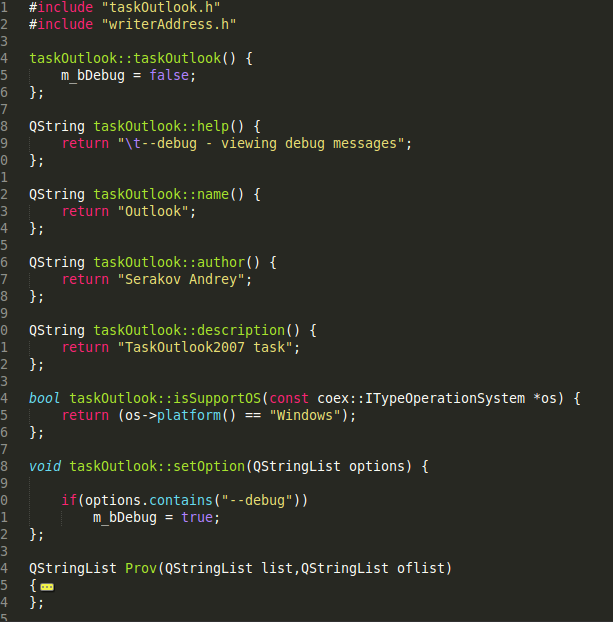
\includegraphics[width=0.6\linewidth]{Outlook}}
\caption{ Функции для описания плагина и функции для контроля выполнения плагина }
\label{Outlook:Outlook}
\end{figure}

\begin{figure}[h!]
\center{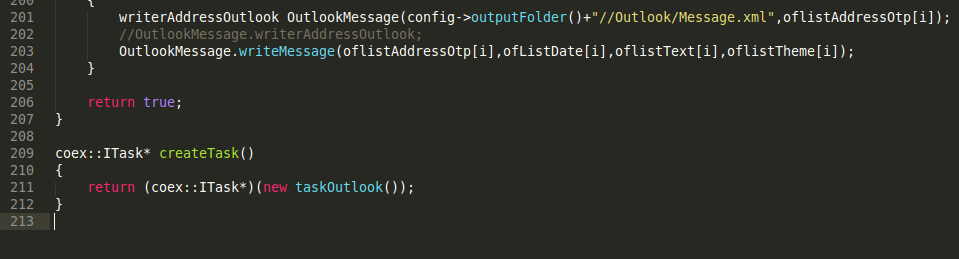
\includegraphics[width=0.6\linewidth]{Outlook2}}
\caption{ Функция для контроля выполнения плагина в программном комплексе }
\label{Outlook2:Outlook2}
\end{figure}



